	\chapter{Contrôle}
	Le système est contrôlé par deux microcontrôleurs un \pic ainsi qu'un \dspic. Le \pic se charge de la communication avec le smartphone au travers du module Bluetooth, il utilise ensuite les informations reçues pour contrôler le servomoteur de direction et envoie les informations adéquates au \dspic. Celui ci gère la puissance du moteur Brushless, il pilote l'onduleur triphasé présenté ici: \ref{onduleur}.
		\section{Communication}
			\subsection{Vue d'ensemble}
				Dans notre système, nous disposons de plusieurs appareils \textit{intelligent}, le \pic , le \dspic et le smartphone, afin que l'on puisse profiter au maximum des capacités de chacun, ces éléments doivent communiquer entre eux.
				\subsubsection{Technologies utilisées}
				Nous utilisons plusieurs technologies de communication différentes entre chaque composant.
				\paragraph{Entre le \textit{Smartphone} et le \textit{Module Bluetooth}} Une liaison \textit{Bluetooth Low Nergal} est établie entre le le module Bluetooth HC-05 et le smartphone. Dans notre cas, le téléphone est dit \textit{master} tandis que le module est dit \textit{slave}.
				\paragraph{Entre le \textit{Module Bluetooth} et le \textit{\pic} } Pour communiquer entre le module Bluetooth HC-05 et le \pic, une liaison série est utilisé. Cette liaison utilise deux conducteurs de données appelés TX et RX. La communication s'effectue à un baud rate commun entre les deux appareils. Le port TX d'un appareil est connecté au port RX du second et inversement.
				\paragraph{Entre le \textit{\dspic} et le \textit{\pic}} Entre ces deux composants, nous utilisons une connexion de type \textbf{SPI}. Cette liaison utilise 3 ou 4 conducteurs. Ils sont appelés SLCK (\textsf{Serial Clock}), MISO (\textsf{Master Input Slave Output}), MOSI (\textsf{Master Output Slave Input})  et SS (\textsf{Slave Select}). Le dernier n'étant utile uniquement si il y a plusieurs \textit{slave} dans le système. Dans notre cas, le \pic est \textit{master} et le \dspic est \textit{slave}
				
				\setlength{\unitlength}{1mm}
\begin{figure}
	\begin{picture}(210,45)
	
		\multiput(15,20)(50,0){4}{\oval(30,10)}
		\put(115,40){\oval(30,10)}
		\put(115,25){\line(0,1){10}}	  
		\put(165,0){\oval(30,10)}	 
		\put(165,5){\line(0,1){10}}   
		\multiput(30,20)(50,0){3}{\line(1,0){20}}  
		
	    \put(3,19){Smartphone}
	    \put(59,19){HC-05}
	    \put(105,19){\pic}
	    \put(102,39){Servomoteur}
	    \put(152,19){\dspic}
	    \put(155,-1){Onduleur}
	    
	    \scriptsize
	    \put(34,16){Bluetooth}
	    \put(88,16){Série}
	    \put(140,16){SPI}
	    \put(36,22){<0-255>}
	    \put(85,22){<0-255>}
	    \put(135,22){<100-200>}
	    \put(117,29){PWM}
	    \put(167,9){PWM}
	\end{picture}
	\caption{Diagramme de communication}
\end{figure}
				\subsubsection{Protocole}
				Avant de mettre en place une communication, il faut définir le \textit{langage} dans le quel nous allons parler. Entre le Smartphone et le Module Bluetooth, nous envoyons un octet. Nous avons donc 256 valeurs pour échanger les informations de puissance, de direction et d'effets. Nous avons donc décidé qu'à chaque mise à jour des curseurs de contrôle, des boutons d'effet ou en cas d'overflow du timer de sécurité, un nombre entre 0 et 255 serait envoyé par Bluetooth. On peut donc résumer les différente significations dans le tableau \ref{protocol}.
\begin{table}[h]
	\begin{center}
	
	\begin{tabular}{cc}
		<0>       & Information de connexion \\
		<1>    	  & Non utilisé               \\
		<2-20>    & Contrôle de la direction  \\
		<21-94>   & Non utilisé               \\
		<95-200> & Contrôle de la puissance  \\
		<201-255> & Effets                   
	\end{tabular}
		\end{center}
	\caption{Correspondance entre les valeurs et les fonctions associées}
	\label{protocol}
\end{table}

			\subsection{Application}
			Afin de pouvoir utiliser notre propre protocole, défini ci dessous, et d'avoir notre propre interface graphique nous avons décider de créer notre application de A à N. Pour cela, nous avons utilisé l'outil développer par le MIT, \href{http://ai2.appinventor.mit.edu/}{MIT App Inventor}. Cette outils en ligne permet de créer avec des blocs de simples applications pour smartphone.
		\paragraph{Interface de connexion} Lorsque nous démarrons l'application, nous arrivons sur un écran qui scan et liste les différents périphériques Bluetooth Low Energy à proximité de notre smartphone. Cette vue reprend les éléments développés dans ce tutoriel \cite{tutoBLE} du MIT. Plusieurs options s'offrent à nous, le scan des périphérique ou la connexion à un des périphériques. Lorsque nous nous connectons à un périphérique, nous basculons sur l'écran de commande de l'aéroglisseur.
		\begin{figure}
			\begin{center}
				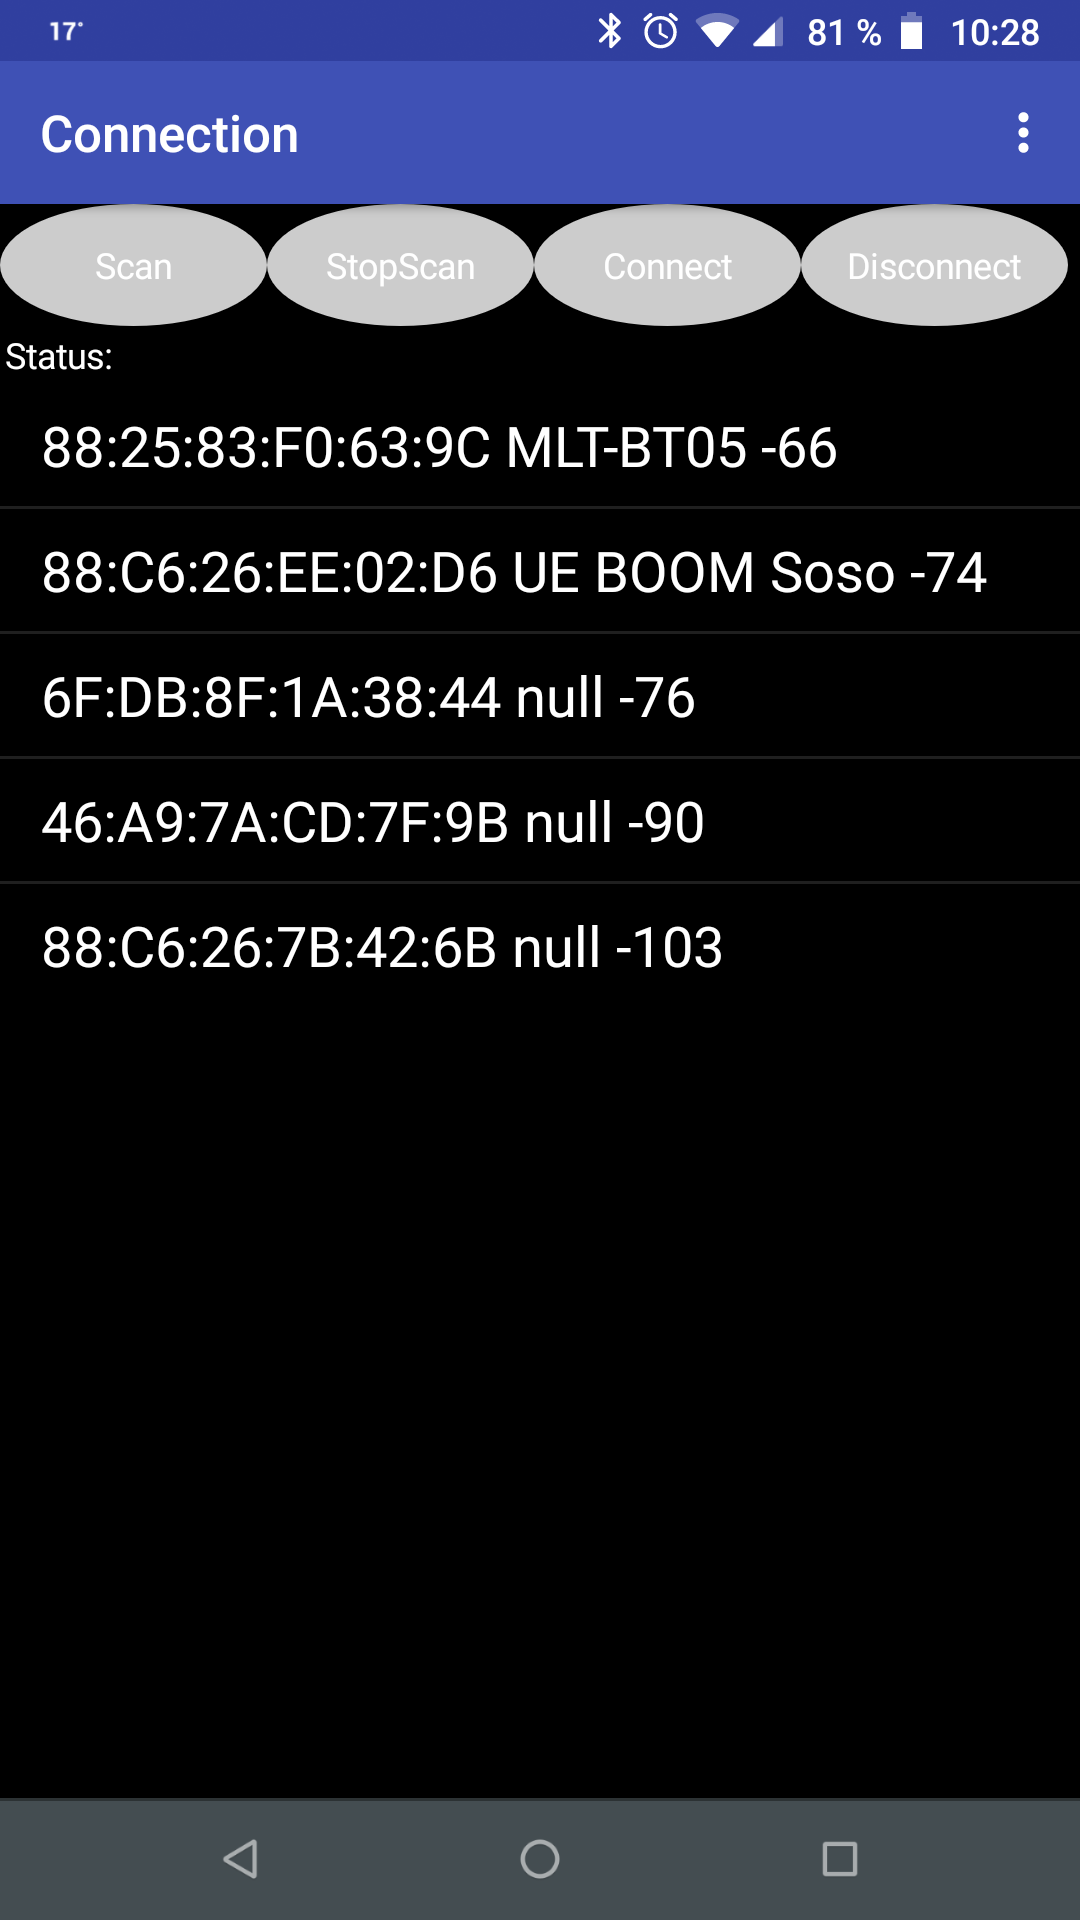
\includegraphics[width=0.3\textwidth]{../Illus/AppConnection.png}
			\end{center}
			\caption{Écran de connexion au périphérique Bluetooth}
		\end{figure}
			\paragraph{Interface de commande} L'écran de commande est composé de deux curseurs, celui de droite contrôlant la puissance et celui de gauche contrôlant la direction. En haut au milieu, il y a un bouton pour se déconnecter et revenir à l'écran d'accueil. En bas de l'écran, une série d'interrupteur permettant l'allumage de différents effets.
			\begin{figure}
		\begin{center}
			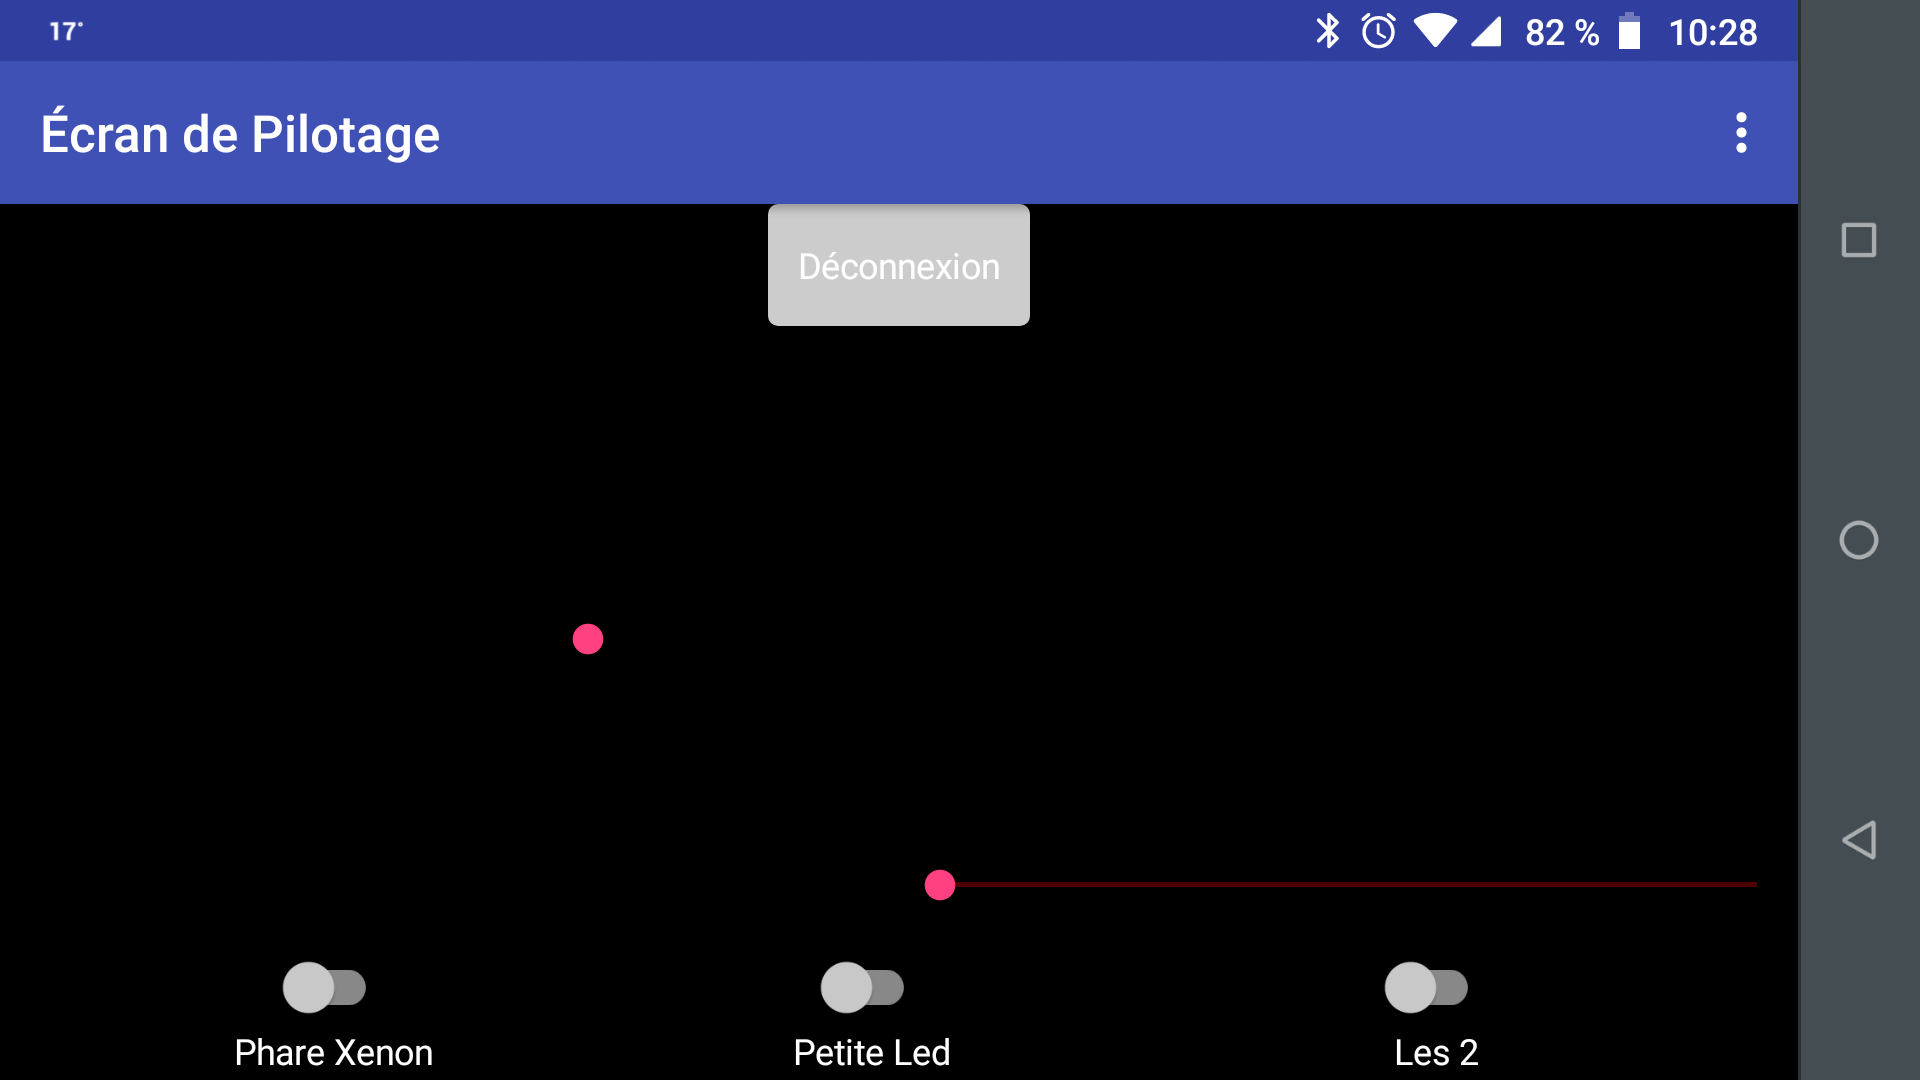
\includegraphics[width=0.6\textwidth]{../Illus/AppPilotage.png}
		\end{center}
			\caption{Écran de pilotage de l'aéroglisseur}
		\end{figure}
		\paragraph{Programmation}
		La programmation sur MIT App Inventor s'effectue avec des blocs. Chaque élément ajouté sur un écran est associé à des blocs fonctionnels. Cette manière de fonctionner ne permet pas de réaliser des applications extrêmement complexes mais permet de réaliser rapidement des interfaces sur smartphone. Notre application ne nécessite pas énormément de choses pour fonctionner, les écrans sont très simples. Nous pouvons résumer le fonctionnement de l'application avec le diagramme suivant: \ref{algoApp}
		\begin{figure}
		\begin{picture}(230,120)
		\scriptsize
			\put(10,50){\framebox(25,10)[c]{\shortstack{Mouvement du\\ curseur Direction}}}
			\put(45,50){\framebox(25,10)[c]{\shortstack{Mouvement du\\ curseur Puissance}}}
			\put(80,50){\framebox(25,10)[c]{Appui sur un effet}}
			\put(115,50){\framebox(25,10)[c]{Fin du timer}}
			\put(150,50){\framebox(25,10)[c]{\shortstack{Appui sur\\ déconnexion}}}

			\put(92.5,80){\line(0,-1){10}}
			\put(22.5,70){\line(1,0){140}}			
		
			\multiput(22.5,50)(35,0){4}{\vector(0,-1){20}}
			\multiput(22.5,20)(35,0){4}{\vector(0,-1){10}}
			\multiput(22.5,70)(35,0){5}{\vector(0,-1){10}}
			\put(162.5,50){\line(0,-1){20}}			
			
			\put(162.5,30){\line(1,0){20}}
			\put(182.5,30){\line(0,1){90}}
			\put(0,10){\line(1,0){127.5}}			
			
			\put(0,75){\vector(1,0){92.5}}			
			
			\put(0,10){\line(0,1){65}}				
			
			\put(10,20){\framebox(25,10)[c]{\shortstack{Envoi de la valeur\\<2-20>}}}
			\put(45,20){\framebox(25,10)[c]{\shortstack{Envoi de la valeur\\<100-200>}}}
			\put(80,20){\framebox(25,10)[c]{\shortstack{Envoi de la valeur\\<201-255>}}}
			\put(115,20){\framebox(25,10)[c]{\shortstack{Envoi de la valeur\\<0>}}}

			
			\put(80,80){\framebox(25,10)[c]{\shortstack{Appui sur\\ connexion}}}
			
			\put(80,100){\framebox(25,10)[c]{\shortstack{Scan}}}
			\put(92.5,100){\vector(0,-1){10}}
			\put(92.5,120){\vector(0,-1){10}}
			\put(110,95){\line(0,1){20}}
			\put(92.5,95){\line(1,0){17.5}}
			\put(92.5,120){\line(1,0){90}}
			\put(92.5,115){\line(1,0){17.5}}
		\end{picture}
			\caption{Algorithme de fonctionnement de l'application}
			\label{algoApp}
		\end{figure}
		\\Chaque fonction ci dessus est assimilable à un bloc de MIT App Inventor. Par exemple, prenons la branche \textit{Mouvement curseur direction}.
		\begin{figure}
			\begin{center}		
				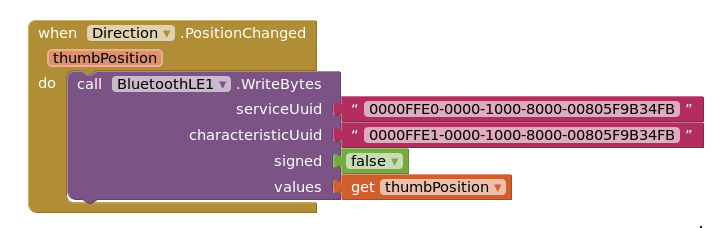
\includegraphics[width=0.5\textwidth]{../Illus/MITBlock.png}
				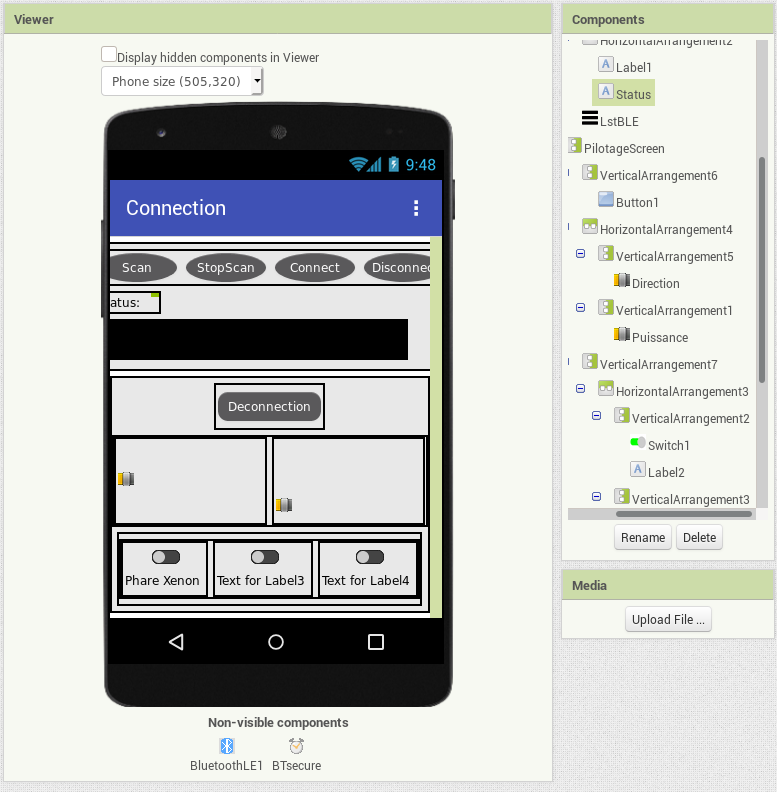
\includegraphics[width=0.2\textwidth]{../Illus/MITScreen.png}
			\end{center}
			\caption{Vues de MIT App Inventor}
		\end{figure}
		Nous pouvons voir les différents éléments constituant notre application, et un exemple de bloc qui réagit au changement de position du curseur pour l'envoyer le la liaison Bluetooth Low Energy.
		\\Les sources du projet de l'application est disponible sur notre dépôt Github ici\cite{git}.
			\subsection{Liaison Bluetooth}
			Après avoir émis les informations de pilotage, il faut les récupérer pour les exploiter. Nous avons donc mis en place une liaison série entre le module Bluetooth HC-05 et le \pic. Cette liaison est déclarée à 9600 bauds.
			\paragraph{Mise en place}La configuration du module \textit{UART} du \pic est réalisée en s'appuyant sur la documentation technique\cite{DatasheetPIC}. On décide les pins que l'on va utiliser, tous les pins utilisés sur les microcontrôleurs sont précisés dans les tableaux \ref{pinoutpic} et \ref{pinoutdspic}.
			
			\insertcode{../../ENUM/Codes/mainpic.c}{73-83,180-182,186-192}{Initialisation de la liaison série sur le \pic}
			
	%interuptuion mise en place lien vers partie du traitenemnt
			\subsection{Liaison SPI}
			La liaison SPI fonctionne comme un registre à décalage. Le \textit{master}, ici le \pic, échange son registre \texttt{SSP1BUF} avec le \textit{slave}, le \dspic, au rythme d'une horloge générée par le \textit{master}.
	\begin{figure}[hb]
		\begin{center}
			\begin{picture}(125,35)
			\tiny
			\multiput(0,10)(75,0){2}{
				\multiput(5,0)(5,0){8}{\framebox(5,5){}}
				\put(23,-2){\vector(1,0){8}}
			}
			
			\put(42.5,10){\line(0,-1){5}}
			\put(82.5,5){\vector(0,1){5}}
			\put(42.5,5){\line(1,0){40}}
			
			\put(7.5,20){\vector(0,-1){5}}
			\put(117.5,15){\line(0,1){5}}
			\put(7.5,20){\line(1,0){110}}
			
			\multiput(55,30)(1.5,2){2}{
				\multiput(0,0)(3,0){5}{
					\put(0,0){\line(1,0){1.5}}				
				}			
			}
			\put(49,27.5){\vector(1,0){29}}
			
			\multiput(55,30)(1.5,0){10}{
					\put(0,0){\line(0,1){2}}				
				}
			\multiput(0,0)(75,0){2}{
				\multiput(3.5,0)(45.5,0){2}{
					\multiput(0,0)(0,3){12}{\line(0,1){1.75}}			
				}
				\multiput(3.5,0)(0,35){2}{
					\multiput(0,0)(3,0){15}{\line(1,0){1.75}}			
				}
			}
			
			\put(20,32){\pic}
			\put(100,32){\dspic}
			\put(59,24.5){SCK}
			\put(59,17){MISO}
			\put(59,2.5){MOSI}
			\end{picture}
		\end{center}
		\caption{Fonctionnement du SPI}
	\end{figure}
			\subsubsection{Sur le \pic}
			\paragraph{Mise en place}La configuration du module \textit{UART} du \pic est réalisée en s'appuyant sur la documentation technique\cite{DatasheetPIC}. On décide les pins que l'on va utiliser, tous les pins utilisés sur les microcontrôleurs sont précisés dans le tableau \ref{pinoutpic}.
			\insertcode{../../ENUM/Codes/mainpic.c}{95-107}{Initialisation de la liaison SPI sur le \pic}
			\subsubsection{Sur le \dspic}
			\paragraph{Mise en place}La configuration du module \textit{UART} du \dspic est réalisée en s'appuyant sur la documentation technique \cite{DatasheetDSPIC} et \cite{DatasheetDSPIC30} . On décide les pins que l'on va utiliser, tous les pins utilisés sur les microcontrôleurs sont précisés dans le tableau \ref{pinoutdspic}.
			\insertcode{../../ENUM/Codes/maindspic.c}{133-147}{Initialisation de la liaison SPI sur le \dspic}
			
		\section{Fonctionnement}
		Dans les tableaux \ref{pinoutdspic} et \ref{pinoutpic} sont réunis tous les pins utilisés sur chacun de nos microcontrôleurs. Cette répartition n'a pas forcément de logique et s'appuie sur les éléments contenus dans les datasheets ou sur des exemples trouvés sur internet.\\
		\begin{table}[hb]
			\begin{multicols}{2}
			\begin{center}
			
			
			\begin{footnotesize}
			\begin{tabular}{r|ccc|l}
				VCC		& 1 &   & 20 & GND \\ 
				  		& 2 &   & 19 & PRGD \\ 
				Effet	& 3 &   & 18 & PRGC \\ 
				MCLR 	& 4 &   & 17 & Arrêt d'urgence \\ 
				Servo 	& 5 &   & 16 &   \\
				 Effet	& 6 &   & 15 &   \\ 
				(Enable)	& 7 &   & 14 & SDO \\ 
				UVFB 	& 8 &   & 13 & SDI \\ 
				BTTX 	& 9 &   & 12 & BTRX \\ 
				SCK 	& 10&   & 11 & Effet   \\ 
				\end{tabular} 
				\\ \texttt{Enable} non utilisé, il permet d'éteindre l'alim
			\end{footnotesize}
				
			
			\caption{Plan de branchement sur le \pic}
			\label{pinoutpic}
		
			
			\begin{footnotesize}
				\begin{tabular}{r|ccc|l}
				MCLR 	& 1 &    & 28 & AVDD 	\\ 
				  		& 2 &    & 27 & AVCC 	\\ 
				  		& 3 &    & 26 & PWM1H	\\
				  		& 4 &    & 25 & PWM1L	\\ 
				  		& 5 &    & 24 & PWM2H	\\ 
				  		& 6 &    & 23 & PWM2L  	\\ 
				 		& 7 &    & 22 & PWM3H  	\\ 
				GND 	& 8 &    & 21 & PWM3L  	\\ 
				  		& 9 &    & 20 & VDD 	\\ 
				  		& 10 &   & 19 & GND 	\\ 
				  		& 11 &   & 18 & SDI 	\\ 
				  		& 12 &   & 17 & SDO 	\\ 
				VDD 	& 13 &   & 16 & SCK 	\\ 
				  		& 14 &   & 15 & Zero Cross\\ 
				\end{tabular} 
			\end{footnotesize}
			\caption{Plan de branchement sur le \dspic}
			\label{pinoutdspic}
			\end{center}
			\end{multicols}
		\end{table}

		\begin{figure}[!h]
			\begin{picture}(210,85)
			\tiny
			
			\newsavebox{\diamo}
				\savebox{\diamo}
				  (20,15){% definition
				  \put(-10,0){\line(5,2){10}}
				  \put(-10,0){\line(5,-2){10}}
				  \put(10,0){\line(-5,2){10}}
				  \put(10,0){\line(-5,-2){10}}
				}
				
				%centre
				\put(90,85){\oval(20,8)}
				\put(86.5,84){Début}
				
				\put(90,81){\vector(0,-1){5}}
				\put(80,68){\framebox(20,8)[c]{\shortstack{Initialisation\\(PWM,Timer,Com)}}}
				
				\put(90,68){\line(0,-1){15}}
				%droite
				\put(50,53){\line(1,0){120}}	
						
				\multiput(110,53)(30,0){3}{\vector(0,-1){4.75}}			
				\multiput(110,37)(30,0){3}{\usebox{\diamo}}
				\multiput(110,40.75)(30,0){3}{\vector(0,-1){4.75}}
				\multiput(100,27.75)(30,0){3}{\framebox(20,8)[c]{}}
				\multiput(110,27.75)(30,0){3}{\line(0,-1){7.75}}
	
				\put(185,60){\vector(-1,0){95}}
				\put(185,60){\line(0,-1){50}}
				
				\put(110,20){\line(1,0){60}}
				\put(140,20){\line(0,-1){10}}
				\put(140,10){\line(1,0){45}}
	
				\put(20,43){\line(1,0){60}}	
				\put(50,53){\line(0,-1){10}}		
				
				%gauche
				\multiput(20,43)(30,0){2}{\vector(0,-1){4.75}}			
				\multiput(20,27)(30,0){2}{\usebox{\diamo}}
				\put(80,43){\vector(0,-1){16.25}}
				\multiput(20,30.75)(30,0){2}{\vector(0,-1){4.75}}
				\multiput(10,17.75)(30,0){3}{\framebox(20,8)[c]{}}
				\multiput(20,17.75)(30,0){3}{\line(0,-1){7.75}}
				
				\put(20,10){\line(1,0){60}}		
				\put(0,0){\line(1,0){50}}			
				\put(0,0){\line(0,1){65}}	
				\put(0,65){\vector(1,0){90}}			
				\put(50,10){\line(0,-1){10}}
				
				
				%cadre
				\multiput(95,49)(87,0){2}{
					\multiput(0,0)(0,-3){9}{\line(0,-1){1.5}}			
				}
				\multiput(95,49)(0,-27){2}{
					\multiput(0,0)(3,0){29}{\line(1,0){1.5}}			
				}
				%texte
	
				\put(42,33.5){\shortstack{Mode\\Arrêt d'Urgence?}}
				\put(15,33.5){\shortstack{Mode\\Défaut BT?}}
				\put(45,18.5){\shortstack{Effet 1\\Puissance 0\\Servo droit}}
				\put(15,18.5){\shortstack{Effet 2\\Puissance 0\\Servo droit}}
				\put(72,18){\shortstack{Mise à jour Effet\\Envoi Puissance\\Mise à jour Servo}}
				
				\put(102,44){\shortstack{Arrêt d'Urgence}}
				\put(135.5,42){\shortstack{Réception\\BT}}
				\put(165.5,42.25){\shortstack{Timer\\overflow}}
				\put(102,30){\shortstack{Activer Mode\\Arrêt d'urgence}}
				\put(130.5,30){\shortstack{Décodage \\Mise à Jour des états}}
				\put(163,30){\shortstack{Activer Mode\\Défaut BT}}
				
				\put(96,25){Interruptions}
			\end{picture}
			\caption{Algorithme simplifié du code du \pic}
			\label{algoPic}
		\end{figure}
			\paragraph{Sur le \pic} Le déroulement du programme sur le \pic suit le schéma représenté sur le diagramme \ref{algoPic}. On peut y voir une phase d'initialisation, configurant les différents registres dont on a besoin. La boucle principale, représenté sur la gauche de l'algorithme, se charge de l'affichage et de la mise à jour de tous les procédés. (Position du servomoteur, Puissance de la propulsion au travers du \dspic, gestion des \textbf{effets non pyrotechnique} \emph{(les effets pyrotechniques étant interdits dans le cahier des charges)}). Cette boucle est interrompue par les fonctions \textit{d'interruptions} gérant l'arrivée de nouvelles informations ou de défauts, ces fonctions sont représentées à droite de l'algorithme. Le contenu ainsi que le fonctionnement des fonctions est détaillé fonction par fonction dans les paragraphes suivants.
			%\paragraph{Sur le \dspic}
			\subsection{Contrôle du servomoteur}
				\paragraph{Fonctionnement}
			Un servomoteur est un moteur asservi en position ou en vitesse. Grâce à un signal de commande caractérisé plus loin, le moteur rejoint une position angulaire ou une vitesse donnée. L'emploi de ce type d'actionneur est simple, une alimentation fixe en 0-5V et un signal de commande permet la réalisation simple de système contrôlé angulairement. Le mot "servo" ne vient pas de cerveau qui signifierait intelligent mais du latin \emph{servus} qui signifie esclave. Il s'agit donc d'un moteur esclave, plus précisément un moteur asservi.
			
				\paragraph{Commande}Le signal de commande employé pour contrôlé les servomoteurs est un signal de type PWM (Power Width Modulation, Modulation à Largeur d'Impulsion). La largeur de l'impulsion correspond à une position donnée. Le signal est un signal électrique de période 20ms, toutes les 20ms, le moteur doit recevoir un signal de commande pour s'aligner correctement. La largeur de l'impulsion varie généralement entre 0.5 et 3ms. La largeur d'impulsion fait varier proportionnellement l'angle de sortie ou la vitesse. Par exemple, si une impulsion de 0.75ms correspond à un angle de $0^{\circ}$ et une impulsion de 2.25 à un angle de $180^{\circ}$. Pour obtenir un angle de $66^{\circ}$, il faut une impulsion de 1.3ms.  
			
				\paragraph{Création du signal de commande} Afin de générer le signal de commande pour le servomoteur, nous allons utiliser le \pic. Ce composant programmable nous permettra de générer le signal comportant une impulsion de largeur variable toutes les 20ms. En jouant sur le rapport cyclique, nous jouons sur la largeur de l'impulsion. Cette largeur d'impulsion sera contrôlée par les information transmise sur la liaison \textit{Bluetooth}. Dans la datasheet du \pic \cite{DatasheetPIC}, on peut voir la formule suivante sur la période du PWM.
				$$ PWM_{period}=(PR2+1)\times 4 \times T_{osc} \times TMR2_{prescaler}$$
				$$ 20*10^{-3}=(PR2+1) \times 4 \times \frac{1}{4*10^{6}} \times 128$$
				$$ PR2=\left(\frac{20*10^{-3}}{128*10^{-6}} \right)-1=155.25$$
				On choisit donc une valeur de \texttt{PR2} de 155. Maintenant, il nous reste à déterminer les valeurs pour obtenir des impulsions de la bonne largeur.
				$$ PulseWidth=[PWM3DCH:PWM3DCL<7-6>]\times T_{osc} \times TMR2_{prescaler}$$
				$$ PulseWidth_{min}=[PWM3DCH:PWM3DCL<7-6>]\times \frac{1}{4*40^{6}} \times 128$$
				$$ PulseWidth_{max}=[PWM3DCH:PWM3DCL<7-6>]\times \frac{1}{4*40^{6}} \times 128$$
				En faisant des essais sur le servomoteur, on détermine expérimentalement les valeurs montrées dans le tableau \ref{PWMval}.
				\begin{table}[h]
				\begin{center}
					\begin{tabular}{c|c|c}
					
					Angle du servo & Valeur de \texttt{PWM3DCH:PWMDCL} & Largeur de l'impulsion \\ 
					\hline 
					$0\deg$ & 8 & 0.256ms \\
					$90\deg$ & 40 & 1.28ms \\
					$180\deg$ & 80 & 2.56ms \\ 
					
					\end{tabular} 
					\caption{Valeurs de la PWM}
					\label{PWMval}
				\end{center}
				\end{table}
				Dans notre code nous n'utilisons pas le registre \texttt{PWM3DCL}, on se contente de charger une valeur entre 2 et 20 dans le registre \texttt{PWM3DCH}, on perd en précision mais cela ne pose pas de soucis. Nous arrivons tout de même à avoir suffisamment de niveau pour remplir le cahier des charges.
				\begin{tcolorbox}[center,width=0.9\textwidth, colframe=red!90!orange, colback=orange!25, arc=3mm,boxrule=1mm, sharp corners=east,title=Note]
			L'aéroglisseur n'ayant pas pu être réalisé, les valeurs maximum et minimum sont l'amplitude maximum du servo, celui ci balaie donc les 180$\deg$ de sa course. Dans le système réel il aurait fallu les limiter afin que la dérive ne rentre pas en butée contre la structure de l'aéroglisseur. Voir \ref{vues}.\\
			Si il faut réduire l'amplitude de battement du servo, il est possible que l'on ai plus assez de niveaux en utilisant uniquement le registre \texttt{PWM3DCH} et il aurait fallut utiliser l'intégralité des registres.
  			\end{tcolorbox}
			
			\subsection{Contrôle des effets}
			Afin d'ajouter un peu de beauté sur notre projet, nous avons décidé d'y ajouter quelques LEDs, c'est ce que nous appelons "effet". Contrôlé par l'application, à chaque réception du caractère associé à l'effet on "inverse" l'état de l'effet.
			\insertcode{../../ENUM/Codes/mainpic.c}{130-143}{Contrôle des effets sur le \pic}
			\begin{tcolorbox}[center,width=0.9\textwidth, colframe=red!90!orange, colback=orange!25, arc=3mm,boxrule=1mm, sharp corners=east,title=Note]
			Les effets définis dans le code ne sont pas forcément les effets définitifs, ils sont ainsi car je n'avais pas plus de LEDs à disposition.
  			\end{tcolorbox}
			
			\subsection{Sécurité}\label{secu}
			Notre projet pouvant s'avérer devenir un objet glissant incontrôlé, il faut mettre en place différents organes de sécurité.
			
				\subsubsection{Batterie faible}
				Comme décrit précédemment (voir \ref{UVBF}) une batterie de type Li-Po ne doit pas se décharger en dessous d'un certain seuil. Le circuit décrit permet de détecter le passage sous ce seuil, mais encore faut-il faire quelque chose. Lorsque le signal en provenance du circuit de protection des sous tensions est à l'état bas, nous empêchons toutes communications et nous déclenchons un effet visuel pour avertir l'utilisateur.
				\insertcode{../../ENUM/Codes/mainpic.c}{226-231}{Gestion de la sous tension batterie sur le \pic}
				\subsubsection{Perte de connexion}
				La perte de connexion entre l'Aéroglisseur est le Smartphone peut être un problème dangereux, personne n'a envie de se confronter à un aéroglisseur fou avec une hélice tranchante en rotation. Pour éviter ce soucis, l'application Bluetooth envoie au minimum un caractère toutes les 100ms, voir paragraphe \ref{algoApp}, soit à cause d'une action de l'utilisateur, il envoi donc l'information, soit en cas d'overflow d'un timer, ce timer déclenche l'envoi d'un 0 toutes les 100ms. À chaque réception d'un nouveau caractère, un timer sur le \pic est réinitialisé. Si le timer déclaré sur le \pic overflow, une interruption est déclenchée, elle met la valeur de la puissance à 0, le servomoteur de direction droit et allume un effet visuel.
				\insertcode{../../ENUM/Codes/mainpic.c}{84-94,113-115,143-146}{Gestion de la perte de connexion sur le \pic}
				
				\subsubsection{Arrêt d'urgence}\label{AU}
				Un arrêt d'urgence, sous la forme d'un \textbf{gros bouton rouge}, n'est pas envisageable pour notre système, car encore une fois devoir d'approcher d'un aéroglisseur fou n'est pas une partie de plaisir Nous avons donc pensé à une corde qui \textit{pend} à l'arrière de l'engin. En tirant sur cette corde, on active un système de bouton qui permet de mettre l'aéroglisseur en un mode de sécurité. Un jumper présent sur la carte permet de servir de commutateur. Sur un front descendant, nous déclenchons une interruption semblable à celle définie ci dessus.
				
				\insertcode{../../ENUM/Codes/mainpic.c}{152-156}{Gestion de l'arrêt d'urgence sur le \pic}
				
				\subsubsection{Hiérarchisation des "erreurs"}
				Le traitement des erreurs a lieu en plusieurs phases. Il y a la phase de détection qui peut avoir lieu avec des interruptions ou pas. Les erreurs sont donc hiérarchisé comme dans le tableau suivant:
				\begin{table}
				\begin{center}
					\begin{tabular}{r|l}
					Priorité&Type d'erreur\\
					\hline
					 1 & Arrêt d'urgence 	\\ 
					 2 & Sous tension batterie 	\\ 
					 3 & Perte de connexion Bluetooth	\\
					 4 & Fonctionnement normal	\\
					\end{tabular} 
					\end{center}
				\end{table}
				Nous traitons en premier lieu le \texttt{global fail} lié à l'arrêt d'urgence, puis la sous tension, la perte de connexion et enfin le fonctionnement sans erreur. Cette hiérarchisation ne pose pas de problèmes étant donné que les différences de traitement réside principalement dans la nature de l'effet avertissant l'utilisateur
			\subsection{Contrôle à partir des données Bluetooth}
			Maintenant que chaque fonctionnalité a été présentée, nous pouvons tout réunir. Le fonctionnement global de notre code s'articule autour de deux parties de code: l'interruption déclenchée par l'arrivée d'information sur le module Bluetooth et la boucle principale.
			\paragraph{Réception Bluetooth} La réception d'information provenant du module Bluetooth sur la liaison série déclenche une interruption. Lorsque cela arrive, le programme en cours est \textit{immédiatement} stoppé et exécute le contenu de la routine associée. Dans notre cas, la routine associée permet de récupérer la valeur reçue, cette valeur est \textit{décodée} en suivant le protocole défini ici: \ref{protocol}.
			\begin{itemize}
			\item[$\bullet$] Si la valeur reçue correspond à une mise à jour des effets, les variables \texttt{eff1} et \texttt{eff2} sont mises à jour, ici complémentée. 
			\item[$\bullet$] Si la valeur reçue correspond à une mise à jour de la direction, on met à jour la variable \texttt{ang}, qui représente la valeur à mettre dans le registre de gestion de la PWM. En effet, pour cette action, il n'y a aucun traitement à faire, c'est pour cela que les valeurs sont ainsi sur le curseur de l'application.
			\item[$\bullet$] Si la valeur reçue correspond à une mise à jour de la puissance de propulsion, un traitement est effectué avant d'être envoyé dans la variable \texttt{puissance} qui sera envoyé sur le \textit{SPI}. On réajuste les valeurs reçues afin qu'elles correspondent par la suite à la valeur nécessaire pour contrôler les signaux PWM contrôlant l'onduleur. On effectue donc une transformation linéaire pour passer d'une valeur entre 95 et 200 à une valeur entre 41 et 230.
			$$ x\in [95;200];y\in [41;230] \Rightarrow y=1.8*x-130 $$
			\label{picmain}
			\item[$\bullet$] Si la valeur ne correspond à rien ou est un 0, le message ne sert juste à montrer que l'application est toujours connectée pour des raisons de sécurité, comme expliqué au paragraphe \ref{secu}.		
			\end{itemize}			 
			\insertcode{../../ENUM/Codes/mainpic.c}{111-142}{Réception Bluetooth sur le \pic}
			\paragraph{Boucle principale} Dans la boucle, on retrouve la gestion des modes. Notre système comporte quatre "modes":
			\begin{itemize}
			\item[$\bullet$] Le mode normal (\texttt{fail=0 et gfail=0}), il s'agit du mode par défaut et normal du système. Dans ce cas, la consigne en puissance est transmise au \dspic, la PWM contrôlant le servo et les effets sont mis à jour toutes les 10ms.
			\item[$\bullet$] Le mode défaut (\texttt{fail=1 et gfail=0}), il s'agit du mode "sans connexion". Il n'y a aucune information qui est arrivé sur la liaison Bluetooth depuis trop longtemps. On met l'aéroglisseur en sécurité, la consigne de puissance est nulle et la dérive est dans une position droite et on fait clignoter un effet afin d'avertir l'utilisateur. Dès que la connexion Bluetooth est rétablie, le système peut repasser en mode normal. Un exemple de cette situation pourrait être que l'aéroglisseur est trop loin du pilote ou encore que le pilote a fermer l'application. Dans ce cas, l'aéroglisseur s'arrête automatiquement.
			\item[$\bullet$] Le mode sous tension de batterie (signal bas sur \texttt{RC3}).Dans ce cas, la consigne en puissance est transmise au \dspic, la PWM contrôlant le servo et un effet averti l'utilisateur.
			\item[$\bullet$] Le mode défaut global (\texttt{fail=1 et gfail=1}), ce mode n'est activé que lorsque l'arrêt d'urgence a été activé, lorsque l'on a arraché le jumper de sécurité. On met l'aéroglisseur en sécurité, la consigne de puissance est nulle et la dérive est dans une position droite et on fait clignoter tous les effets afin d'avertir l'utilisateur qu'il s'agit d'un autre défaut que ci dessus. En revanche dans ce mode, le redémarrage est impossible. Il faut débrancher la batterie, remettre en place le jumper de sécurité et réalimenter le système. Dans ce mode, toutes nouvelles informations sont bloquées, plus aucun événement ne peut déclencher une interruption. 
			\end{itemize}
			\insertcode{../../ENUM/Codes/mainpic.c}{216-247}{Boucle principale du \pic}
			
			
			\subsection{Contrôle de l'onduleur}			
			\begin{tcolorbox}[center,width=0.9\textwidth, colframe=red!90!orange, colback=orange!25, arc=3mm,boxrule=1mm, sharp corners=east,title=Note]
			Cette partie a été réalisée durant la période de fermeture de l'école. N'ayant pas eut un oscilloscope et un moteur brushless à disposition, les codes n'ont pas été testé sur système réel. Le projet a été simulé sur \textit{MPLABxIDE}. Malheureusement, ce simulateur présente de nombreux défauts comme un manque de stabilité et des visualisations de sortie très limitées, notamment sur la durée des simulations. Les valeurs calculées ne sont donc pas forcément adaptées\\
  			Comme vous pourrez le voir dans la partie \ref{real}, un système de LED est ajoutée pour visualiser les sorties PWM. 
  			\end{tcolorbox}
  			Le contrôle de l'onduleur, présenté paragraphe \ref{onduleur}, est effectué par le \dspic . Il s'agit donc de créer 6 signaux  PWM pour contrôler chaque transistor de la structure globale. De plus, ces signaux doivent être cadencé afin de créer un champ tournant mais aussi synchroniser avec la méthode de \textit{Back EMF}.
  			\paragraph{Mise en place des signaux PWM}
  			La mise en place des signaux PWM sur le \dspic a été effectué en suivant le tutoriel \cite{PWMds}. On obtient 6 signaux PWM. Les signaux sont liés 2 à 2, il y a un signal PWM et son complément. On a donc PWMxL et PWMxH pour chaque sortie 1,2 et 3.On retrouve cette répartition sur la figure \ref{imgPWM}.
  			\begin{figure}[hb]\begin{center}
	  			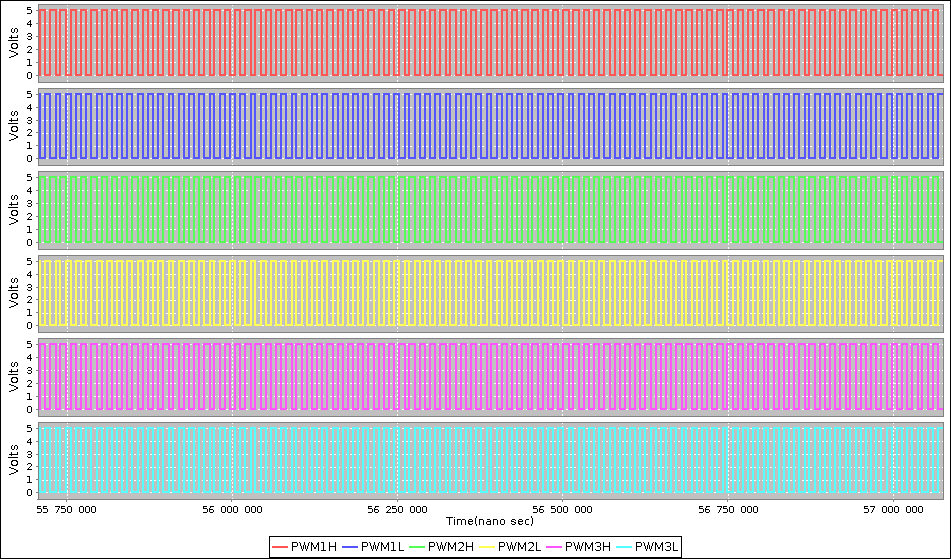
\includegraphics[width=0.9\textwidth]{../Illus/pwm100.png}
	  			\caption{Simulation des signaux PWM}
	  			\label{imgPWM}
	  			\end{center}
  			\end{figure}
  			L'onduleur doit être piloté avec des signaux de commandes d'une fréquence entre 16kHz et 20kHz. Aidons nous de la datasheet \cite{DatasheetDSPIC} pour calculer la fréquence de notre PWM. Nous avons notre générateur de PWM configuré en \textit{Free Running Mode}, on utilise donc la formule suivante:
  			$$T_{PWM}=\frac{1}{F_{PWM}}=T_{CY}\times (PTPER+1)\times PTMR_{Prescaler}$$
  			$$\frac{1}{16*10^{3}}=\frac{4}{7.37*10^6}\times (PTPER+1)\times 1$$
  			$$PTPER=\frac{7.37*10^6}{4 \times 16*10^3}-1=114.15625 $$ 
  			\insertcode{../../ENUM/Codes/maindspic.c}{78-101}{Mise en place des signaux PWM sur le \dspic}
  			On peut maintenant calculer la résolution du PWM afin de savoir quel consigne devons nous lui donner. On utilise donc la formule de la datasheet:
  			$$\frac{\log\left(2 \times \frac{F_{CY}}{F_{PWM}}\right)}{\log 2}=7.84$$
  			On peut donc commander le signal PWM entre 0 et $2^7.84$ soit 230.
			\paragraph{Contrôle depuis les informations du \pic}
			Les informations en provenance du \pic sont entre 41 et 230. Elles sont mises en forme sur le \pic, voir paragraphe \ref{picmain}.
			\paragraph{Relation entre PWM et pulsation}
			%Voir si c'est ici ou dans la partie du BLDC	
			$$ $$
  			\paragraph{Séquençage}
  			Afin de générer un champs tournant, on doit alterner l'activation et la désactivation des différentes sorties actifs à l'état haut ou à l'état bas. La séquence utilisée est décrite dans la note d'application \cite{AN857}.
  			\insertcode{../../ENUM/Codes/maindspic.c}{102-132}{Gestion de l'ordre des phases sur le \dspic}
  			On obtient donc les signaux suivant:
  			\begin{figure}[hb]\begin{center}
	  			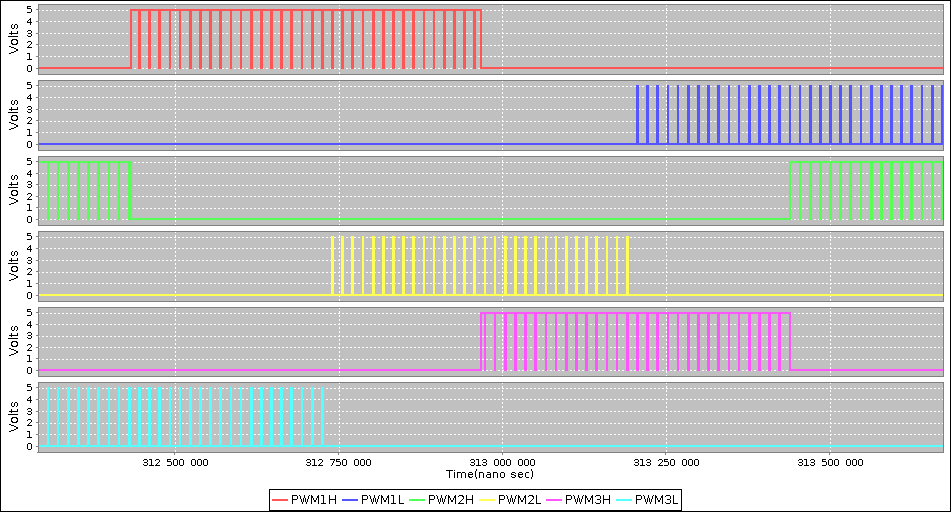
\includegraphics[width=0.9\textwidth]{../Illus/PWMCadence2015.png}
	  			\caption{Simulation des signaux PWM cadencés}(L'échelle de temps n'est pas correcte, afin de pouvoir observer tous les signaux sur le simulateur)
	  			\label{imgPWM}
	  			\end{center}
  			\end{figure}
  			\paragraph{Fonctionnement général}
  			L'algorithme simplifié du code du \dspic est représenté figure \ref{algodsPic}. On y retrouve les phases d'initialisations, d'interruption et la boucle principale comme pour dans le code \ref{algoPic} pour le \pic .
  			\begin{figure}[!h]
			\begin{picture}(210,85)
			\tiny				
			
			\newsavebox{\diamon}
				\savebox{\diamon}
				  (20,15){% definition
				  \put(-10,0){\line(5,2){10}}
				  \put(-10,0){\line(5,-2){10}}
				  \put(10,0){\line(-5,2){10}}
				  \put(10,0){\line(-5,-2){10}}
				}
				%centre
				\put(90,85){\oval(20,8)}
				\put(86.5,84){Début}
				
				\put(90,81){\vector(0,-1){5}}
				\put(80,68){\framebox(20,8)[c]{\shortstack{Initialisation\\(PWM,Timer,Com)}}}
				
				\put(90,68){\line(0,-1){15}}
				%droite
				\put(50,53){\line(1,0){120}}	
						
				\multiput(80,53)(30,0){4}{\vector(0,-1){4.75}}			
				\multiput(80,37)(30,0){4}{\usebox{\diamon}}
				\multiput(80,40.75)(30,0){4}{\vector(0,-1){4.75}}
				\multiput(70,27.75)(30,0){4}{\framebox(20,8)[c]{}}
				\multiput(80,27.75)(30,0){4}{\line(0,-1){7.75}}
	
				\put(185,60){\vector(-1,0){95}}
				\put(185,60){\line(0,-1){50}}
				
				\put(80,20){\line(1,0){90}}
				\put(125,20){\line(0,-1){10}}
				\put(125,10){\line(1,0){60}}
	
				\put(12,43){\line(1,0){50}}	
				\put(50,53){\line(0,-1){10}}		
				
				%gauche
				\multiput(12,43)(30,0){2}{\vector(0,-1){4.75}}			
				\multiput(12,27)(30,0){2}{\usebox{\diamon}}
				\put(62,43){\line(0,-1){33}}
				\multiput(12,30.75)(30,0){2}{\vector(0,-1){4.75}}
				\multiput(2,17.75)(30,0){2}{\framebox(20,8)[c]{}}
				\multiput(12,17.75)(30,0){2}{\line(0,-1){7.75}}
				
				\put(12,10){\line(1,0){50}}		
				\put(0,0){\line(1,0){50}}			
				\put(0,0){\line(0,1){65}}	
				\put(0,65){\vector(1,0){90}}			
				\put(50,10){\line(0,-1){10}}
				
				
				%cadre
				\multiput(65,49)(117,0){2}{
					\multiput(0,0)(0,-3){9}{\line(0,-1){1.5}}			
				}
				\multiput(65,49)(0,-26){2}{
					\multiput(0,0)(3,0){39}{\line(1,0){1.5}}			
				}
				%texte
	
				\put(35,33.25){\shortstack{power\\<PowerTarget}}
				\put(6,33.25){\shortstack{power\\>PowerTarget}}
				\put(37,20.5){\shortstack{power++}}
				\put(7,20.5){\shortstack{power- -}}
				
				\put(75,42.5){\shortstack{Front sur\\entrée}}
				\put(105,44){\shortstack{Timer 2}}
				\put(135.5,42){\shortstack{Réception\\SPI}}
				\put(166,44){\shortstack{Timer 3}}
				\put(75,30){\shortstack{Changement\\ au secteur 0}}
				\put(105,30){\shortstack{Changement \\de secteur}}
				\put(132,30){\shortstack{Mise à jour \\de powerTarget }}
				\put(163,30){\shortstack{Mise à jour de la\\ pulsation}}
				
				\put(67,24){Interruptions}
			\end{picture}
			\caption{Algorithme simplifié du code du \dspic }
			\label{algodsPic}
		\end{figure}
		
		\insertcode{../../ENUM/Codes/maindspic.c}{190-231}{Boucle principale sur le \dspic}
		
		\section{Réalisation}\label{real}
			\begin{tcolorbox}[center,width=0.9\textwidth, colframe=red!90!orange, colback=orange!25, arc=3mm,boxrule=1mm, sharp corners=east,title=Note]
			La réalisation a été faite avec les \textit{moyens du bord}. Cette section présente quelques fonctionnalités fonctionnelles sur plaquette d'essais.
  			\end{tcolorbox}
  			\begin{figure}[hb]
				\begin{center}						
				\includegraphics[width=0.5\textwidth]{../Illus/real.png}
				\begin{picture}(0,0)
				\linethickness{0.3mm}
				\textcolor{red}{
					\put(-15.5,11){\framebox(4,18)}%dsPIC
					\put(-60,23){\framebox(9,4)}%PIC
					\put(-60,41){\framebox(12,4)}%BT
				}
				\textcolor{blue}{
					\put(-29,36){\framebox(22,22)}%servo
					\put(-13,2){\framebox(3,5)}%LED
					\put(-54,28){\framebox(3,3)}%LED
					\put(-62,8){\framebox(5,9)}%Fil AU
				}
				\textcolor{green}{
					\put(-37,10){\framebox(14,14)}%PWM
					\put(-56,8){\framebox(5,9)}%Fil bat
					\put(-90,49){\framebox(25,17)}%ARDuino				
				}
				\end{picture}
			\end{center}
			\caption{Prototype de travail pour le projet}
			En rouge les microcontrôleurs et le Bluetooth. En bleu, les éléments réels qui serait tel quel sur le projet. En vert, les solutions alternatives.
		\end{figure}
  			Nous pouvons résumer en 2 catégories les composants sur la plaquette d'essais.
  			
  			\begin{table}[hb]\begin{center}
	  			\begin{tabular}{c|c}
	  			Composants réellement présent & Composant Alternatif\\
	  			\hline
	  			\pic & PWM (jeux de LED) \\ 
	  			\dspic & Fil sous tension batterie (Fil relié au VCC ou au GND)\\
	  			 Servo &  Alimentation (Arduino) \\
	  			 Module Bluetooth &\\ 
	  			 LEDs &\\
	  			 Fil d'arrêt d'urgence &\\
	  			
	  			\end{tabular}\end{center}
  			\end{table}
 Ce montage permet de réaliser et de tester quelques fonctionnalités du projet. Vous pouvez consulter une vidéo de ce montage en fonctionnement ici: \url{youtube.com}
